\chapter{Sensitivity and noise in gravitational wave detectors}
\label{c:instrumentation}

\section{Interferometer response}

The effect that an interferometer has on a means of readout (e.g. a photodetector) as some variable is modulated is termed the \emph{response}. The most important response to consider in gravitational wave interferometry is the arm cavity differential degree of freedom's response to the beam splitter's output port. The response varies as a function of frequency depending on the interferometer topology and its light storage time. For instance, in a Michelson interferometer the dARM response is typically flat for frequencies below the arm cavity pole, and decaying \checkme{at a rate proportional to frequency} above. At higher frequencies, less light can be stored as the cavity cannot build up sufficient light power due to mirror loss and round-trip time. This effect is shown in \note{Figure XXX} for different end test mass reflectivities and in \note{Figure XXX} for different arm cavity lengths.

In order to calculate a response function for a set of optics, it is necessary to understand the propagation of a light field through vacuum and through optics.

\subsection{Interferometer fields}
* Intro to field equations of Fabry-Perot. Perhaps generalise to Michelson? Point reader towards analytical calculation of DRFPMI (Ken Strain paper).

We define the field amplitude of light across dimension $x$ as:
\begin{equation}
  \label{eq:field-amplitude}
  E = E_0 \text{e}^{\text{i} kx},
\end{equation}
for initial amplitude $E_0$ and wavenumber $k = \frac{2 \pi}{\lambda}$, where $\lambda$ denotes wavelength. Upon transmission through an optic, the transmitted field is equal to the input field, $E_{\text{in}}$, scaled by the optic's field transmissivity, $t$:
\begin{equation}
  \label{eq:transmitted-field}
  E_{\text{t}} = tE_{\text{in}}.
\end{equation}
The reflected field is similarly scaled by the optic's field reflectivity, $r$:
\begin{equation}
  \label{eq:reflected-field}
  E_{\text{r}} = \text{i}rE_{\text{in}}.
\end{equation}
Note the presence of complex coefficient $\text{i}$, equivalent to a multiplication by $\text{e}^{\text{i} \frac{\pi}{2}}$. This shows that the phase difference between reflected and transmitted fields is $\frac{\pi}{2}$, which is required for energy conservation. We choose to apply this phase shift to the reflected field by convention (see Appendix\,\ref{a:reflection-phase}).

\subsubsection{Simple cavities}
\note{Make sure this is consistent with PDH description etc. later, i.e. reflected field is E7 or whatever, etc.}

\begin{figure}
  \centering
  \includegraphics[width=\columnwidth]{graphics/generated/from-svg/20-fabry-perot.pdf}
  \caption{\label{fig:fabry-perot}\FP{} cavity with its mirror input and output coefficients. Coefficients $a_1$ and $a_5$ are for the fields incident upon the cavity from either side, whilst $a_4$ and $a_8$ are for the fields leaving the cavity on either side. Coefficients at the outputs of the \FP{} can be calculated from inputs $a_1$ and $a_5$. The mirrors in the cavity are separated by free space through which the fields leaving each mirror's inside surface propagate.}
\end{figure}

Combining Equations \ref{eq:field-amplitude}, \ref{eq:transmitted-field} and \ref{eq:reflected-field} allows us to determine the field amplitude at different ports of a collection of mirrors. Combinations of mirrors produce \emph{optical cavities}, which possess the property that they can, under certain conditions, accumulate light power. If we take the simplest of examples, the two-mirror \FP{} cavity (see Figure\,\ref{fig:fabry-perot}), we can determine the fields coefficients present at the output nodes of the mirrors to be:

\begin{equation}
  \label{eq:fabry-perot-coefficients-1}
  \begin{split}
    a_1 &= it_1 a_0 + r_1 a_5, \\
    a_3 &= it_2 a_2, \\
    a_4 &= r_2 a_2, \\
    a_6 &= r_1 a_0 + it_1 a_5.
  \end{split}
\end{equation}

Similarly, the coefficients at the input nodes within the cavity can be determined from the output nodes of the opposite mirrors and the separation $D$:
\begin{equation}
  \label{eq:fabry-perot-coefficients-2}
  \begin{split}
    a_2 &= a_1 \text{e}^{\text{i} kD}, \\
    a_5 &= a_4 \text{e}^{\text{i} kD}, \\
  \end{split}
\end{equation}

Note the lack of a field input from the right side of the cavity in Figure\,\ref{fig:fabry-perot}. In general this field is present and has a small effect on the coefficients, but in gravitational wave detectors it is typically small by design. As this additional term adds mathematical complexity but not significant additional clarity, it has been neglected.

The coefficients in Equations \ref{eq:fabry-perot-coefficients-1} and \ref{eq:fabry-perot-coefficients-2} can be used to determine the field amplitude at different points of the interferometer. As there is only one input field in this example, the coefficients can be reduced to depend only on $a_0$, $r_1$ and $r_2$, $t_1$ and $t_2$ and $D$. The light reflected from the \FP{} is an important field to know as this is used in many experiments to assist with interferometer sensing and control. Coefficient $a_6$ determines the reflected field, but this depends on $a_0$ and $a_5$, the latter being one of the coefficients inside the cavity. Coefficient $a_5$ can have terms progressively substituted as follows:
\begin{equation}
  \label{eq:fabry-perot-reflected-coefficient}
  \begin{split}
    a_5 &= a_4 \text{e}^{\text{i} kD} \\
        &= a_2 r_2 \text{e}^{\text{i} kD} \\
        &= a_1 r_2 \text{e}^{\text{2i} kD} \\
        &= r_2 \left( it_1 a_0 + r_1 a_5 \right) \text{e}^{\text{2i} kD}, \\
  \end{split}
\end{equation}
where we find that the equation for $a_5$ depends on itself. This shows how the cavity operates: on each subsequent round trip, the cavity field is enhanced with addition field in the form of light transmitting through the first mirror. The field builds up until the amount of light entering the cavity is equal to the amount leaving. We can manipulate Equation\,\ref{eq:fabry-perot-reflected-coefficient} to show this:
\begin{equation}
  a_5 = a_0 \frac{it_1 r_2 \text{e}^{2ikD}}{1 - r_1 r_2 \text{e}^{2ikD}},
\end{equation}
where it is clear to see that the cavity coefficient depends on the input coefficient $a_0$. The coefficient representing the reflected light from the interferometer is then just $a_5$ scaled by $t_1$:
\begin{equation}
  a_6 = a_0 \left( r_1 - \frac{t_1^2 r_2 \text{e}^{2ikD}}{1 - r_1 r_2 \text{e}^{2ikD}} \right).
\end{equation}

With $a_6$ expressed in terms of $a_0$, we can then calculate the reflected field amplitude as a function of the input field. The output field as a function of input field $E_{\text{in}}$ is then simply:
\begin{equation}
  \label{eq:fabry-perot-field}
  \begin{split}
    E_{\text{out}} &= a_6 E_{\text{in}} \\
                   &= E_{\text{in}} \left( r_1 - \frac{t_1^2 r_2 \text{e}^{2ikD}}{1 - r_1 r_2 \text{e}^{2ikD}} \right).
  \end{split}
\end{equation}
The term in brackets in Equation\,\ref{eq:fabry-perot-field} is termed the \emph{transfer function} of the cavity, i.e. the ratio of the output field with respect to the input field. This is an important figure of merit for cavities and will be especially important in the later chapters of this work.

\subsubsection{Cavity figures of merit}
\note{FSR, finesse, etc.}

\subsubsection{Signal sidebands}
\note{Talk about signal sidebands ON THE CARRIER ONLY (see G.H. thesis p58)}

The field due to motion of a mirror $\Delta x$ at a distance $x$ can be determined by combining Equations \ref{eq:field-amplitude} and \ref{eq:reflected-field}. As the light must travel distance $2x$ to get to and from the optic, the field picks up a factor of $\text{e}^{2\text{i}k \left( x + \Delta x \right)}$ in phase and a factor of $r$ in amplitude:
\begin{equation}
  E_{\text{r}} \left( x \right) = r E_0 \text{e}^{2\text{i} k \left( x + \Delta x \right)}.
\end{equation}
For clarity, we can express the constant $x$ term as a static phase representing the carrier, separated from $\Delta x$ via the wave number:
\begin{equation}
  \label{eq:field-amplitude-phase}
  E_{\text{r}} \left( t \right) = r E_0 \text{e}^{\text{i} \left( 2 \omega_0 t + k \Delta x\right)}.
\end{equation}
It is possible to express any particular motion in the form of a series of sinusoidal functions. Expressing mirror motion as a single frequency sinusoid modulating the impinging field, we see:
\begin{equation}
  \label{eq:field-phase-modulation}
  E_{\text{r}} \left( t \right) = E_0 \text{e}^{\text{i} \left(\omega_0 t + m \cos{\left( \omega t \right)} \right)},
\end{equation}
where we introduce $m$ as the \emph{modulation depth}, a dimensionless number expressing the strength of the mirror motion. Note that we have neglected for now the reflection term $r$. With some algebraic manipulation involving Bessel functions, we can express this as \cite{Freise2010}:
\begin{equation}
  \label{eq:field-phase-bessel}
  E \left( t \right) = E_0 \text{e}^{\text{i} \omega_0 t} \sum^{\infty}_{n=-\infty} \text{i}^n J_{n} \left( m \right) \text{e}^{\text{i} n \omega t}.
\end{equation}
When $m$ is $0$ all Bessel functions $J_{n}$ are $0$ except the first, which is $1$; this shows that the field contains only the carrier component when there is no external modulation applied by a moving mirror. Conversely, when a non-zero modulation index and signal frequency is present, there exists a sum of sinusoidal functions as a product of the carrier, which we call \emph{signal sidebands}. For small modulation depths $m \ll 1$, Equation\,\ref{eq:field-phase-bessel} can be approximated to:
\begin{equation}
  \label{eq:field-phase-mod-expanded}
  E = E_0 \text{e}^{\text{i} \omega_0 t} \left( 1 - \frac{m^2}{4} + \text{i} \frac{m}{2} \left( \text{e}^{-\text{i} \omega t} + \text{e}^{\text{i} \omega t} \right) \right).
\end{equation}
Here it is clear to see the presence of upper and lower sidebands at frequencies $\omega_0 \pm \omega$.

Amplitude modulation has a similar but not identical effect to phase modulation. Devices such as piezoelectric transducers for trimming laser outputs can perform amplitude modulation on a light field, and the effect can be expressed again in terms of the modulation depth and frequency:
\begin{equation}
  E = E_0 \text{e}^{\text{i} \omega_0 t} \left( 1 + m \cos{\omega t} \right),
\end{equation}
and we can manipulate this expression to show the presence of exactly one upper and one lower sideband:
\begin{equation}
  \label{eq:field-amp-mod}
  E = E_0 \text{e}^{\text{i} \omega_0 t} \left( 1 + \frac{m}{2} \text{e}^{\text{i} \omega t} + \frac{m}{2} \text{e}^{-\text{i} \omega t} \right).
\end{equation}

There is an interesting caveat to highlight here: if there are infinitely many phase modulation sidebands for a given modulation depth, is the phase modulation constant? To resolve this apparent inconsistency it is useful to remember that each Bessel function in the series can be of different sign, such that the sum of all Bessel functions in Equation\,\ref{eq:field-phase-bessel} \checkme{has magnitude equal to the modulation depth}. A \emph{phasor diagram} is useful to visualise this effect. The first four phase modulation sidebands are shown alongside the resultant vector in Figure XXX.

\note{RECREATE TOBIN'S ANIMATION FROM https://dsp.stackexchange.com/questions/2284/why-are-sidebands-generated-in-am-and-fm}

\subsubsection{Signal detection}
When signals are measured by a photodetector, only amplitude modulation can be detected directly. Although the field impinging upon the photodetector contains phase modulation, the photodetector's stray capacitance acts as a filter to remove this effect from the output signal; in essence, the photodetector only sees the time averaged field. A piezoelectric transducer modulating a laser crystal can be readily witnessed on a photodetector, but to access mirror motion encoded as phase modulation, special techniques are required.

In general, phase modulation measurement techniques fall into two broad categories: \emph{heterodyne} detection, and \emph{homodyne} detection. With heterodyne detection, one or more laser frequencies are used in addition to the carrier which have different properties such that they follow a different path to the detector. At the detector, a comparison can be made between the paths taken by the heterodyne fields, where the difference in amplitude and phase can offer insight into the motion of the interferometer's optics. In homodyne detection, the carrier is itself used as a reference, by mixing some light from one part of the interferometer with light from another. If this is conducted in a particular way, it can be a powerful technique to measure phase modulation without requiring carefully controlled heterodyne fields.

Both heterodyne and homodyne techniques will be discussed in greater detail later on.

%\subsubsection{Heterodyne detection}
%Add RF sidebands that don't resonate, schnupp asymmetry, etc...

%\subsubsection{Homodyne detection}
%pick off a bit of carrier light with a DARM offset...

\subsubsection{Numerical simulation tools}
Recall the reflection term $r$ we ignored earlier. Light propagating within an interferometer will collect reflection and transmission terms from each mirror it encounters. A photodetector placed at a port of the interferometer will then see light with amplitude and phase information representing the path it has taken through the interferometer. We have shown this effect in a trivial example involving a \FP{} cavity with one input, but the same mathematics can be used to represent any interferometer. For anything beyond the simplest of examples, we typically employ numerical simulation tools to perform the tedious calculations involved in obtaining the output signals from interferometers, with the packages Finesse \cite{Freise2004} (not to be confused with \emph{cavity} finesse) and Optickle \cite{Evans2012} being popular choices within the field of gravitational wave interferometry.

\section{Limiting noise sources in detectors}
Quantum noise, thermal noise (since if you push QN low enough, you run into thermal), possibly mention others (Newtonian noise - why ET will be under ground, etc.)

\subsection{Measurement noise in gravitational wave interferometry}
Gravitational wave interferometry is ultimately a matter of signals and noise. The term ``signal'' simply refers to a wanted pattern of oscillations representing a particular variable of interest. ``Noise'', on the other hand, is unwanted oscillations that appear at the signal measurement device. The measurement of any signal necessarily entails the measurement of some noise, and so it does not make sense to talk about signal without talking about noise.

\subsubsection{\label{sec:snr}Signal to noise ratio}

Part of scientists' jobs, both experimental and theoretical, is to design experiments and apparatus in such a way as to maximise the ratio of signal power, $S$, to noise power, $N$, in the region of interest. This is the \emph{signal-to-noise} ratio (SNR),
\begin{equation}
  \text{SNR} = \frac{S}{N}.
\end{equation}
In engineering circles the standard representation of signal to noise is in units of \emph{decibels} (\SI{}{\deci\bel}), defined for signal power as:
\begin{equation}
  \text{SNR}_{\SI{}{\deci\bel}} = 10 \log_{10} \left( \frac{s}{n} \right).
\end{equation}
As this representation is logarithmic, it is a useful for expressing both small and large signals. It is borrowed from engineering circles, and is particularly popular in discussions of electronic filtering.

\subsubsection{Optimal operating point}

In precision measurement, typically an experimentalist can only infer the quantity of an underlying amplitude from a measured power. A simple example is the measurement of mirror displacement in a simple Michelson interferometer \emph{via} the photocurrent output of the photodetector. The wave is composed of the electric and magnetic fields, $E$ and $B$, respectively, each of which can be expressed as a travelling wave:
\begin{align}
  E &= E_0 \text{e}^{\text{i} \left( kx - \omega t \right)}, \\
  B &= B_0 \text{e}^{\text{i}  \left( kx - \omega t \right)},
\end{align}
where $E_0$ and $B_0$ are the initial field amplitudes, $k = \frac{2 \pi}{\lambda}$ is the wave vector, $x$ is the displacement, $\omega$ is the angular frequency and $t$ is time. The intensity $S$ is the product of the two, with the magnetic field weighted by the permittivity of free space $\epsilon_0$ and speed of light in vacuum $c_0$ \checkme{check this is consistent with Living Review p31}:
\begin{equation}
  S = \frac{1}{2} \epsilon_0 \left( E^2 + c_0^2 B^2 \right).
\end{equation}
As the $E$ and $B$ fields are orthogonal, their sum at any point in time and space remains constant. We can therefore state that the wave's intensity is proportional to the square of an ``amplitude'' $A$, expressing the combination of $E$ and $B$:
\begin{equation}
  S \propto A^2.
\end{equation}
Leaving the beam splitter towards the end of each arm, each wave in the Michelson interferometer propagates with amplitude
\begin{equation}
  A = A_{\text{in}} \text{e}^{\text{i} \left( kx - \omega t \right)},
\end{equation}
where $A_{\text{in}}$ represents the field at the beam splitter's input.

A difference in path length between the arms $\Delta x$ leads to a difference in round-trip phase between light returning to the beam splitter. With light of constant amplitude injected into the interferometer, and assuming that the light round-trip time is much quicker than the transient causing a change to the arm lengths, we can look at the superposition of returning light at the beam splitter to determine the change in path length. At the beam splitter's output port, the field superposition becomes:
\begin{equation}
  A_{\text{out}} = \frac{A_{\text{in}}}{2} \text{e}^{\text{i} \left( k \left( x + \frac{\Delta x}{2} \right) - \omega t \right)} + \frac{A_{\text{in}}}{2} \text{e}^{\text{i} \left( k \left( x - \frac{\Delta x}{2} \right) - \omega t \right)},
\end{equation}
where we assume that the path length difference caused by the transient is evenly distributed, differentially, between the two arms. The power measured by a photodetector, $P_{\text{out}}$, is then the field multiplied by its complex conjugate:
\begin{equation}
  \label{eq:mich-p-out}
  \begin{split}
    P_{\text{out}} &\propto \langle A_{\text{out}}^*A_{\text{out}} \rangle \\
                   &= \frac{P_{\text{in}}}{2} \left( 1 + \cos \left( k \Delta x \right) \right),
  \end{split}
\end{equation}
using the fact that $P_{\text{in}} = A_{\text{in}}^2$.

Here we see that a static field $\frac{P_{\text{in}}}{2}$ is present upon the photodetector, independent of the arm length change. In simple experiments, often it is practical to keep the interferometer at an operating point commonly referred to as ``half way up the fringe''. Here, the interferometer's mirrors are nominally positioned such that the output signal is oscillating about the midpoint between crest and trough (see Figure\,\ref{fig:fringe}). As the gradient is steepest at this point, any small changes to the relative arm length of the Michelson interferometer result in a significant difference in power at the photodetector. This operating point, however, is not optimal in terms of \emph{sensitivity} to arm length fluctuations. As discussed in Section\,\ref{sec:snr}, the noise level is just as important as the signal.

%% FIXME: change this plot's x-labels to use wavelength, to fit with the conclusion in the text.
\begin{figure}
  \centering
  \includegraphics[width=\columnwidth]{graphics/generated/from-python/20-fringe.pdf}
  \caption{Fringe.}
  \label{fig:fringe}
\end{figure}

By inspecting Equation\,\ref{eq:mich-p-out}, it is clear to see that there must exist, in cases where there is a signal due to a difference in arm length, a static photodetector power independent of the arm length. This does not contribute any displacement information to the measurement, but does contribute shot noise:
\begin{equation}
  P_{\text{shot, out}} = \sqrt{2 h f_0 P_{\text{in}}},
\end{equation}
where $h$ is Planck's constant, $f_0$ is the light frequency and $P_{\text{in}} = A_{\text{in}}^2$, the power entering the interferometer at the beam splitter. The optimally sensitive operating point is therefore not simply one which maximises the signal gradient, but rather one which maximises the SNR. The SNR is:
\begin{equation}
  \text{SNR} = \frac{P_{\text{out}}}{P_{\text{shot, out}}} = \sqrt{\frac{P_{\text{in}}}{4 h f_0}} \left( 1 + \cos \left(k \Delta x \right) \right).
\end{equation}

The $\Delta x$ term in Equation\,\ref{eq:mich-p-out} is a combination of a static arm length \emph{detuning}\textemdash representing the arm length mismatch required to reach the desired operating point\textemdash and a differential gravitational wave signal $\Delta x_{\text{GW}}$. A suitable choice of $ x_{\text{tune}}$ can remove the majority of the static power present at the output. Setting the slope of the SNR with respect to the tuning to zero,
\begin{equation}
  \frac{\Delta \text{SNR}}{\Delta x_{\text{GW}}} = -k \sqrt{\frac{P_{\text{in}}}{4 h f_0}} \sin \left(k \Delta x\right) = 0,
\end{equation}
we find that maximum SNR is achieved for static tunings 
\begin{equation}
  \Delta x = 0 \text{ mod } \lambda.
\end{equation}
This result shows that the optimal operating point in terms of SNR is at the point where the light from the two arms interferes destructively. While any multiple of $\lambda$ will satisfy the SNR condition as defined, in reality we have not considered laser noise coupling. The more matched the arm lengths are, the lower the laser noise couples to the output port. In reality there are also mismatches in the reflectivities of the mirrors in the arms: this creates an asymmetry called a \emph{contrast defect} which leads to additional shot noise at the output port.

%CHECKME At the output port, light from one arm is transmitted through the beam splitter while the light from the other arm is reflected, and so a reflection phase convention applies (see Appendix\,\ref{a:reflection-phase}). The arm lengths are therefore offset by $\frac{\lambda}{4}$ with respect to one another.

% Section 1.3.1 of Gabriele Vajente's thesis covers this in more detail.

\subsubsection{Root mean square amplitude}

\subsubsection{Spectral density}
In gravitational wave interferometry, a lot of thought and planning typically goes in to the design of the apparatus in order to minimise noise \emph{transients}\textemdash pulses of unwanted noise with finite energy\textemdash such as a door slam\footnote{And, of course, some forms of gravitational wave signal; though it is not the intention of experimentalists to minimise the effect of this particular source.}. Such transients have finite energy over a finite time, and can be entirely characterised\textemdash within measurement error\textemdash by a Fourier transform of the time series in which the event occurred. With sufficient isolation from unwanted transients, the remaining noise sources within the interferometer tend to arise from stationary, random processes, with energy approaching infinity as measurement time approaches infinity. In this circumstance, the Fourier transform of the underlying time-domain signal does not strictly exist. An alternative representation of a noise process is to represent the amount of work it performs per unit time: its power. The \emph{power spectral density} is a representation of the power present within each frequency of a signal in the steady state. This distribution can then be integrated back into a finite, steady state power.

Typically the time evolution of a particular signal is the only data an experimentalist has at their disposal in order to characterise a signal in terms of its spectral density. A true representation of the power spectral density requires, like the measurement of energy spectral density, infinite time. A compromise can be made, however, in order to estimate the power spectral density from a set of Fourier transforms of the time series. By averaging Fourier transforms of various subsets of the data $\left[ t, t + \Delta t \right]$, a power spectral density can be approximated for a particular frequency range, determined by the bounds established by the inverse of the longest and shortest subsets of the time series transformed. While this compromise is typically reasonable in most cases, and indeed essential for any finite measurement, it is unable to exclude the possibility that part of the power spectral density is formed from signal content in frequencies outwith the measured range. Longer time series measurements allow for more averaging of frequency bands, and thus a better approximation to the true power spectral density.

\subsubsection{Bandlimiting}
\note{Nyquist-Shannon sampling theorem, https://en.wikipedia.org/wiki/Bandlimiting}

\subsection{Technical noise}

\subsubsection{Laser frequency noise}
A perfect laser provides output at a single, well defined frequency, or in other words, it has an infinitely narrow linewidth. In reality, such lasers do not exist and instead the output contains spectral impurities. As the laser wavelength is the ``metre stick'' by which we make measurements of length in interferometers, it is very important to ensure that the laser's wavelength, and therefore frequency, is well defined. A well designed laser will get an experimentalist part of the way there, but in most cavity experiments a frequency stabilisation control loop involving optics and electronics is necessary.

Apart from its linewidth, it is possible to represent a laser's frequency noise in terms of its noise spectral density, measurable via some heterodyne technique with a standard spectrum analyser. The effect of laser frequency noise is for a beat signal $V \left( t \right)$ to occur due to overlapping sinusoidal waves:
\begin{equation}
  V \left( t \right) = V_0 \left( t \right) \sin \left[ 2 \pi f_0 + \phi \left( t \right) \right],
\end{equation}
where $V_0 \left( t \right)$ is the beat amplitude and $\phi \left( t \right)$ is the phase difference at time $t$. We can rewrite this in terms of frequency $f \left( t \right)$,
\begin{equation}
  \begin{split}
    f \left( t \right) &= f_0 + \frac{1}{2 \pi} \frac{\text{d} \phi \left( t \right)}{\text{d} t} \\
                       &= f_0 + \Delta f \left( t \right),
  \end{split}
\end{equation}
with $\Delta f \left( t \right)$ the instantaneous frequency fluctuation. The power spectral density arises from the autocorrelation between a frequency fluctuation at time $t$ and another at time $t + \Delta t$, which can be expressed in the form:
\begin{equation}
  S_{\Delta f} \left( f \right) = 2 \int^{\infty}_{0} \langle \Delta f \left( t \right) \Delta f \left( t + \Delta t \right) \rangle \text{e}^{\left( -\text{i2}\pi f \Delta t \right) \text{d}\Delta t}
\end{equation}



\note{See Neil's thesis p14, https://arran.physics.gla.ac.uk/wp/speedmeter/2016/03/24/update-on-linear-cavity-work, Optics Communications 201 (2002) 391-397, and Applied Optics 49, issue 25, 4801-4807, 2010}

\subsubsection{Laser intensity noise}
\note{describe RIN, etc...}

\subsection{Thermal noise}

\subsection{Quantum noise}

\subsubsection{The Standard Quantum Limit}

\section{Overview of current efforts}
* aLIGO, aVirgo, KAGRA, GEO
* Sensitivity curves for all?

\section{The future of gravitational wave interferometry}

\subsection{Planned upgrades and new facilities}
* Worldwide network of interferometric detectors
* Plans to build/upgrade more (KAGRA, ET, LIGO Voyager, LIGO CE, etc.)
* Space based detectors

\subsection{Surpassing the Standard Quantum Limit}
\subsubsection{Quantum non-demolition}
Give general overview of technique, then explain the Sagnac speedmeter in more detail.

\begin{figure}
  \centering
  \includegraphics[width=\columnwidth]{graphics/generated/from-python/20-sideband-structure.pdf}
  \caption{Sideband structure}
  \label{fig:sideband-structure}
\end{figure}